% Asset ID: AS1VectorsTikZ-004
% Asset type: TikZ diagram
% Suggested file: tikz/AS1VectorsTikZ-004_parallelogram_law.tex
% Source: CCEA AS1-VEC-LO003; Phase 1 Core Theory 5
% Related lesson section: Geometrical interpretation of vector addition
% Purpose: Show the parallelogram law for adding two vectors.
% Boundary note: 2D vectors only.

\documentclass[tikz,border=8pt]{standalone}
\usepackage{amsmath}
\usetikzlibrary{arrows.meta}
\begin{document}
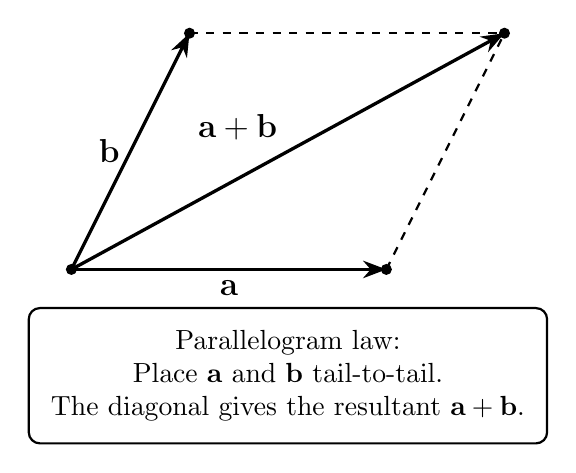
\begin{tikzpicture}[>=Stealth,vector/.style={->, very thick},guide/.style={dashed, thick},resultant/.style={->, very thick},label/.style={font=\large},note/.style={draw, rounded corners, thick, align=center, inner sep=8pt}]
\coordinate (O) at (0,0); \coordinate (A) at (4,0); \coordinate (B) at (1.5,3); \coordinate (C) at (5.5,3);
\draw[vector] (O) -- (A) node[midway, below,label] {$\mathbf{a}$};
\draw[vector] (O) -- (B) node[midway, left,label] {$\mathbf{b}$};
\draw[guide] (A) -- (C); \draw[guide] (B) -- (C);
\draw[resultant] (O) -- (C) node[midway, above left,label] {$\mathbf{a}+\mathbf{b}$};
\fill (O) circle (2pt); \fill (A) circle (2pt); \fill (B) circle (2pt); \fill (C) circle (2pt);
\node[note] at (2.75,-1.35) {Parallelogram law:\\ Place $\mathbf{a}$ and $\mathbf{b}$ tail-to-tail.\\ The diagonal gives the resultant $\mathbf{a}+\mathbf{b}$.};
\end{tikzpicture}
\end{document}
